\chapter{Project Management}
\label{chap:pm}

As stated throughout \see{chap:methodology}, the Iterative model was chosen for this project. All tasks were managed with GitHub projects \see{pm:kanban}. Furthermore, versions were managed with Git for version control \see{pm:version_control} and regular meetings with the project supervisor were scheduled to monitor progress \see{pm:supervisor_meetings}.

\section{GitHub}

\subsection{Kanban Board and Projects}
\label{pm:kanban}

From the beginning, a GitHub project and code repository were created to manage all development and writing tasks \see{fig:kanban}. All tasks were initially added to the backlog and allocated a milestone and label to categorise each task.

Milestones were created for each iteration of the prototype and each section of this document \see{fig:milestones}. Each task would then be assigned a 'To Do' status when selected for development/writing and would progress throughout the other Kanban Board stages until it was marked as 'Done' and closed. This allowed for the effective management of subtasks on a per-milestone and status basis.

An 'In Review' status was added to the Kanban board for tasks that required guidance from the project supervisor \see{pm:supervisor_meetings}.

\newpage
\begin{landscape}
\begin{figure}
    \centering
    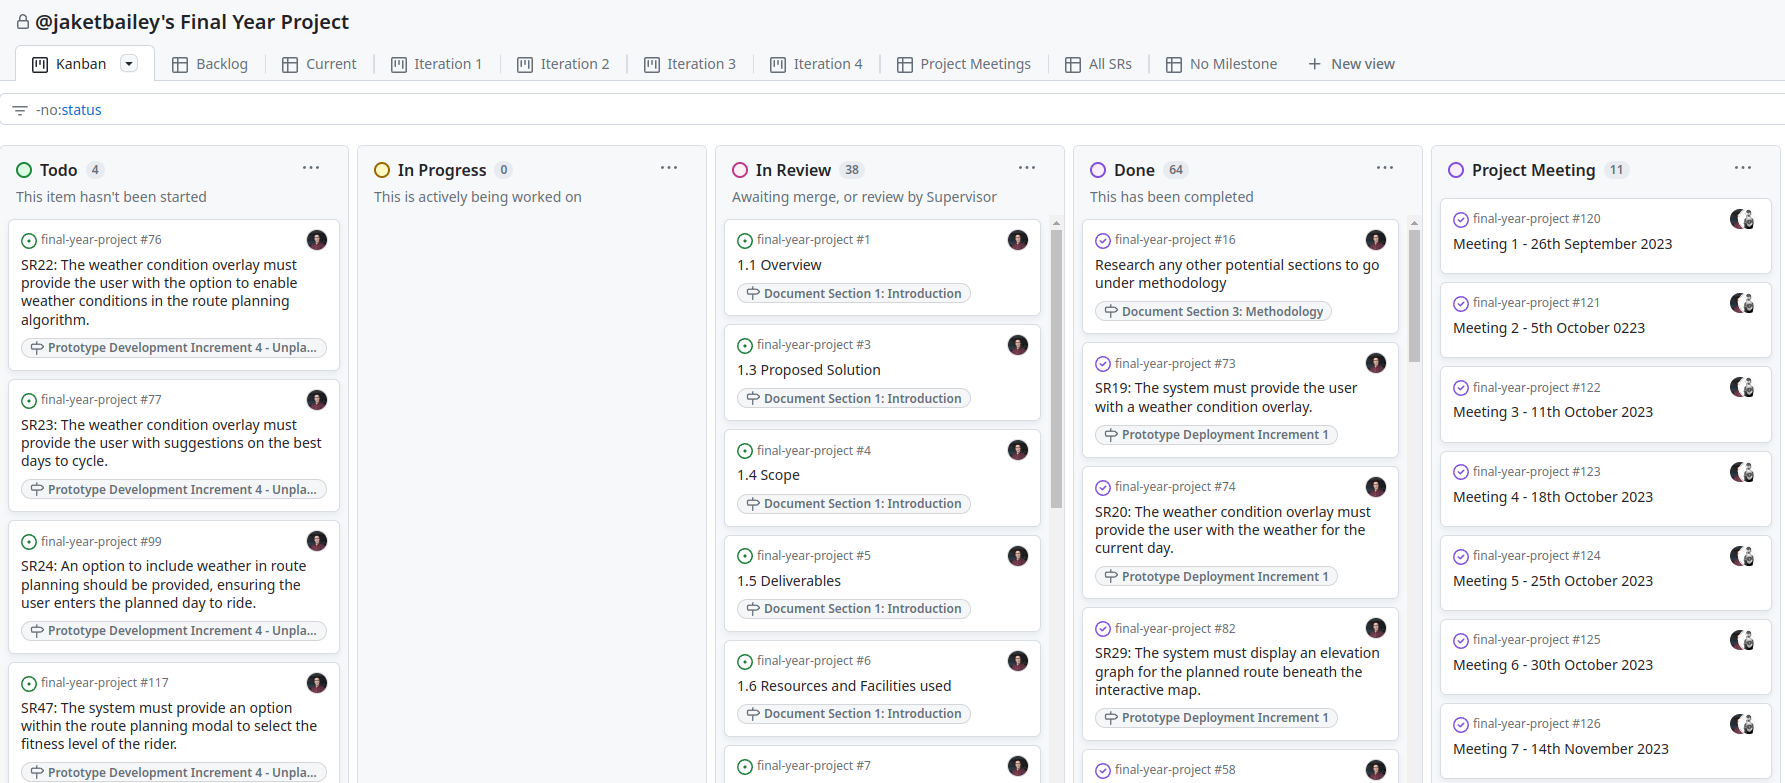
\includegraphics[width=700px]{figures/kanban.png}
    \caption{GitHub Kanban Board}
    \label{fig:kanban}
\end{figure}
\newpage

\begin{figure}
    \centering
    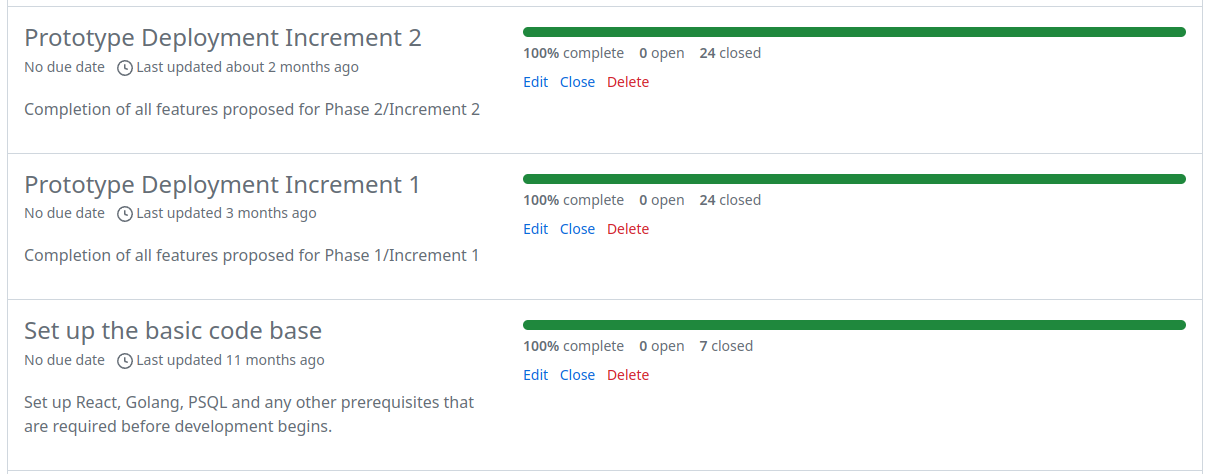
\includegraphics[width=700px]{figures/milestones.png}
    \caption{GitHub Milestones}
    \label{fig:milestones}
\end{figure}
\newpage
\end{landscape}

\subsection{Version Control}
\label{pm:version_control}

GitHub hosted the source code with Git Software Version Management. Using git supported the iterative model where branches and pull requests were created for all code changes and iterations. A git graph was created to demonstrate all significant code changes including the development of core functionalities and system requirements \see{fig:gitgraph}\see{fig:gitgraph2}. Branch-level testing was used with pull requests to automated code change merges. Merges raised conflicts arise between iterations, ensuring the code base remains accurate, forcing the conflict's resolution before changes are made. Commits are also highly valuable during development as they allow code changes to be managed and reversed if needed. 

% \begingroup
\begin{figure}[!ht]
    \centering
    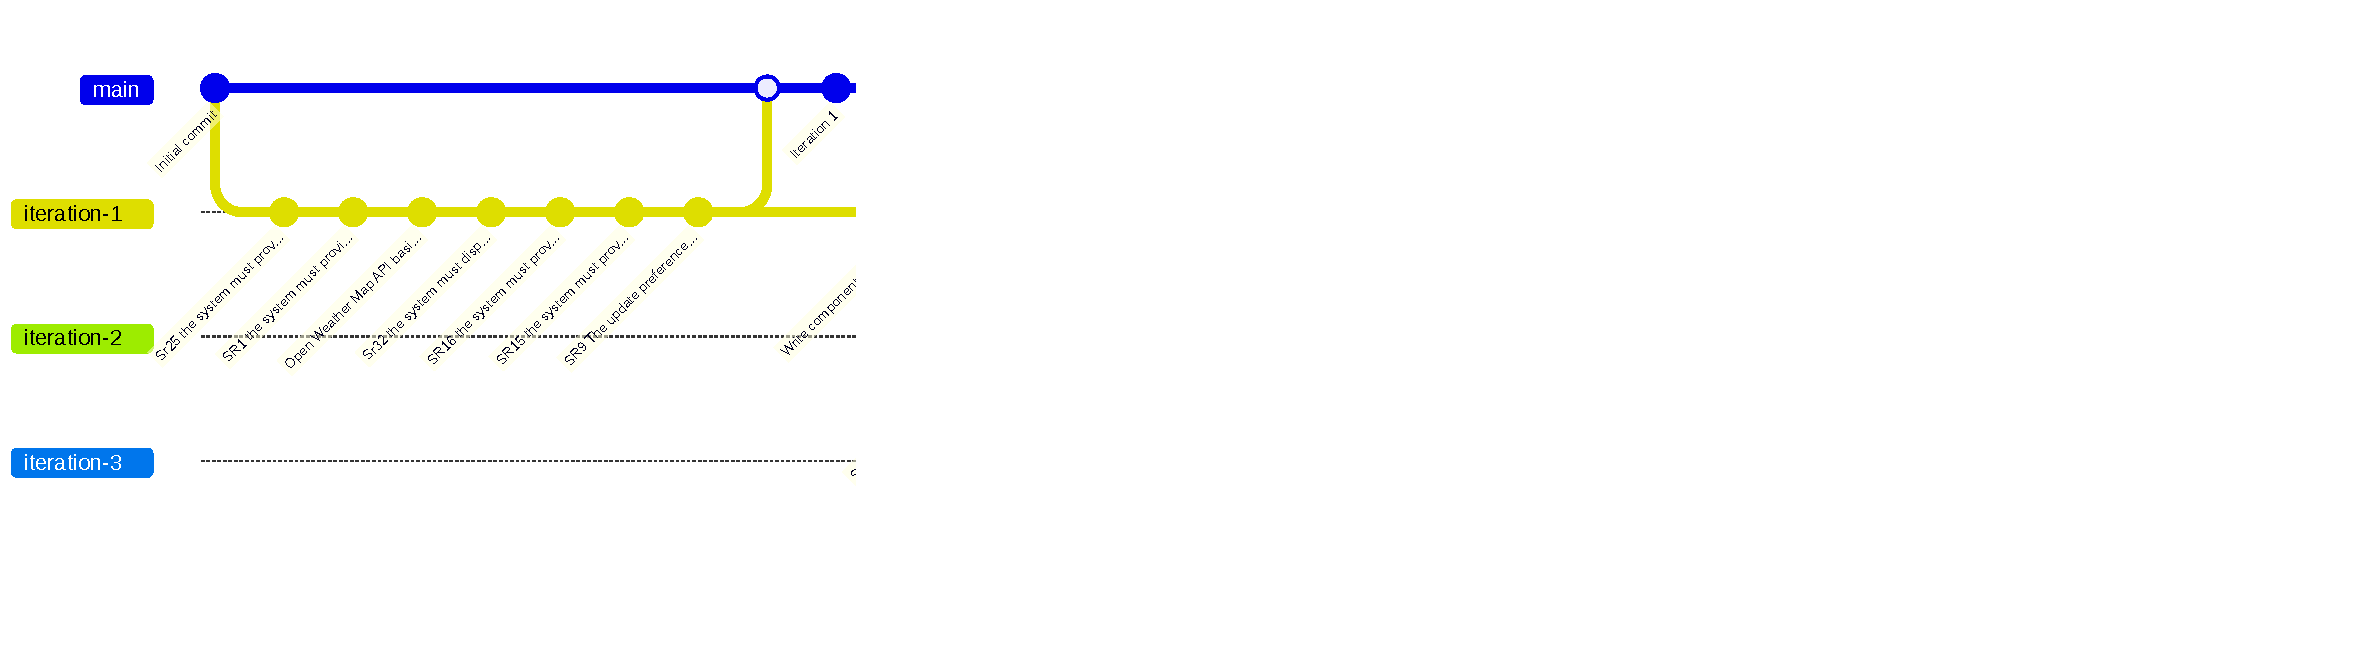
\includegraphics[width=400px]{figures/gitgraph1.pdf}
    \caption{Git Pull Requests and Branches}
    \label{fig:gitgraph}
\end{figure}
\begin{figure}[!ht]
    \centering
    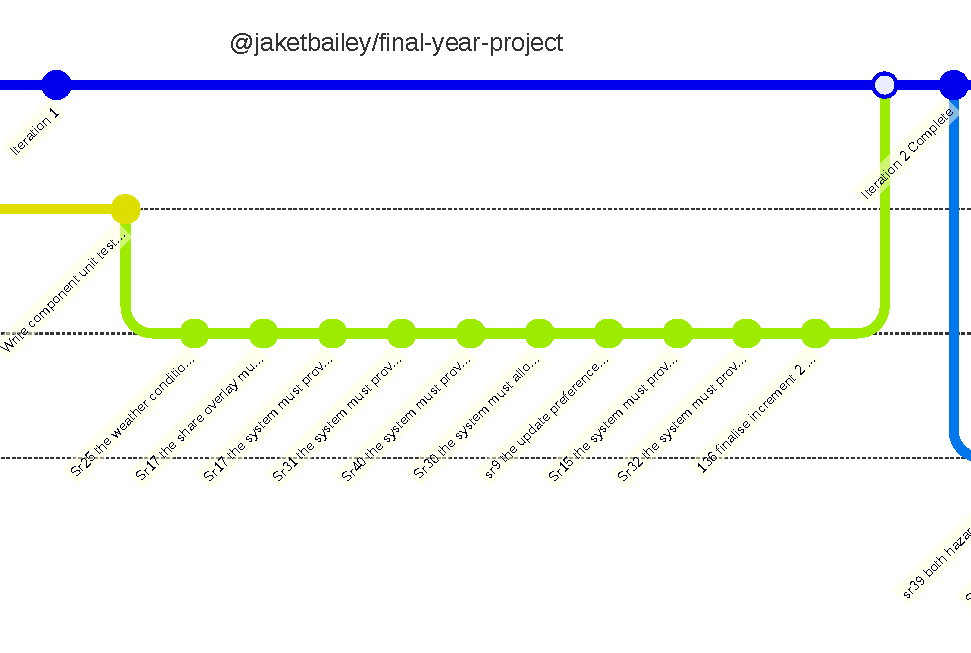
\includegraphics[width=400px]{figures/gitgraph2.pdf}
    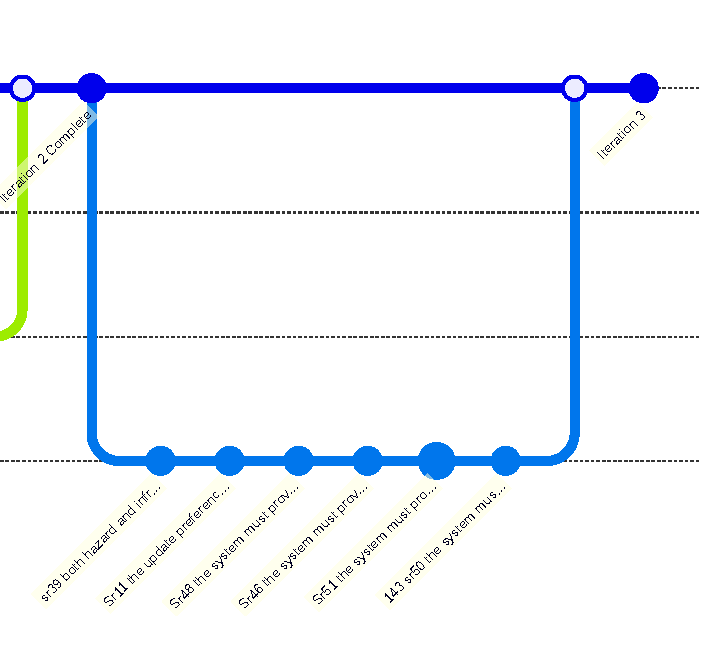
\includegraphics[width=400px]{figures/gitgraph3.pdf}
    \caption{Git Pull Requests and Branches Cont.}
    \label{fig:gitgraph2}
\end{figure}
% \endgroup

\clearpage
\section{Supervisor Meetings}
\label{pm:supervisor_meetings}

Regular meetings were scheduled with the supervisor/client to monitor progress throughout the project. In-person meetings were preferred, however, video conferences were used as a backup. Due to being ahead of schedule, the later meetings comprised primarily of project improvement and personal tutor sessions \see{pm:supervisor_meeting_list}.

\section{Conclusion}
\label{pm:conclusion}

Understanding the project management techniques to implement was key when understanding how the requirements in the would be met \see{chap:requirements}. Between the methodology \see{chap:methodology} and project management plan \see{chap:pm}, it was clear how the user stories could be broken down into smaller, system requirements. Planning was one of the key successes of the project whereby the project was completed ahead of schedule. Further highlighting how the techniques used influenced the elicited requirements.